\chapter{Opis struktury projektu}
\label{cha:opisStruktury}

W tym rozdziale przedstawiona zostanie ogólna struktura projektu, ze szczególnym uwzględnieniem wykorzystanych technologii, organizacji kodu oraz zarządzania danymi. Opisane zostaną hierarchie klas, najważniejsze metody oraz wymagania sprzętowe niezbędne do uruchomienia aplikacji.

\section{Technologie wykorzystane w projekcie}
\label{sec:technologieWykorzystane}
W projekcie wykorzystano szereg technologii umożliwiających tworzenie aplikacji typu desktop z graficznym interfejsem użytkownika, komunikację z relacyjną bazą danych oraz zapewnienie odpowiedniego zarządzania zależnościami i strukturą kodu.

\begin{itemize}
    \item \textbf{Java (OpenJDK 23.0.2)} - język programowania, w którym została napisana aplikacja.
    \item \textbf{JavaFX 23.0.1} - biblioteka graficzna do tworzenia interfejsów użytkownika.
    \item \textbf{FXML + SceneBuilder} - wszystkie widoki interfejsu użytkownika zostały zaprojektowane w Scene Builderze i zapisane jako pliki FXML, co umożliwia rozdzielenie widoków od logiki.
    \item \textbf{JDBC (Java Database Connectivity)} - API służące do komunikacji z relacyjną bazą danych.
    \item \textbf{MySQL Connector/J 8.0.33} - biblioteka umożliwiająca komunikację aplikacji Java z bazą danych MySQL.
    \item \textbf{MySQL} - relacyjna baza danych przechowująca dane dotyczące klientów, pojazdów, zleceń, pracowników itd.
    \item \textbf{phpMyAdmin} - webowe narzędzie do graficznego zarządzania bazą danych MySQL: tworzenia tabel, relacji, testowania zapytań i modyfikacji danych.
    \item \textbf{Maven 3.8.5} - system zarządzania projektem i zależnościami, umożliwiający automatyczne pobieranie bibliotek i budowanie aplikacji.
    \item \textbf{IDE: IntelliJ IDEA 2024.3.3} - środowisko programistyczne używane do pisania kodu, konfiguracji projektu oraz integracji.
\end{itemize}

\newpage
\section{Struktura katalogów i plików}
\label{sec:strukturaKatalogow}
Poniższa struktura katalogów odzwierciedla typowy układ projektu Java z wykorzystaniem narzędzi Maven oraz frameworka JavaFX. Główne foldery zostały podzielone zgodnie z zasadą separacji odpowiedzialności, co ułatwia zarządzanie kodem oraz jego dalszą rozbudowę.
\begin{itemize}
    \item \texttt{src/main/java/project.app} - zawiera kod źródłowy aplikacji podzielony na pakiety zgodnie z rolami komponentów: kontrolery JavaFX (\textbf{controllers}), warstwa dostępu do danych (\textbf{dao}), modele danych (\textbf{model}), interfejsy (\textbf{interfaces}) oraz narzędzia pomocnicze (\textbf{utils}).
    \item \texttt{src/main/resources} - miejsce na zasoby statyczne, takie jak widoki interfejsu użytkownika w formacie FXML (\textbf{project.app}), pliki stylów CSS (\textbf{values}), obrazy (\textbf{images}) oraz plik konfiguracyjny połączenia z bazą danych (\textbf{config.properties}).
    \item Plik na poziomie głównym, taki jak \textbf{pom.xml}, odpowiada za konfigurację projektu Maven, a dokumenty \textbf{README.md} i \textbf{CHANGELOG.md} zawierają opis projektu oraz historię zmian.
\end{itemize}


\begin{figure}[H]
    \label{strukturaKatalogow}
    \centering
    \begin{verbatim}
    |-- SystemZarządzaniaSerwisemSamochodowym/
    |   `-- src/
    |       `-- main/
    |           |-- java/
    |           |   |-- project.app/
    |           |   |   |-- controllers/      <- Kontrolery JavaFX
    |           |   |   |-- dao/              <- Dostęp do danych (JDBC)
    |           |   |   |-- interfaces/       <- Interfejsy
    |           |   |   |-- model/            <- Modele danych
    |           |   |   |-- utils/            <- Klasy pomocnicze
    |           |   |   `- Main.java          <- Klasa główna
    |           |   `-- module-info.java
    |           `-- resources/
    |               |-- images/               <- Zasoby graficzne
    |               |-- project.app/          <- Widoki FXML
    |               |-- values/               <- Pliki CSS
    |               `-- config.properties     <- Plik konfiguracyjny bazy danych
    |-- pom.xml
    |-- CHANGELOG.md                          <- Dziennik zmian
    `-- README.md                             <- Opis projektu
    \end{verbatim}
    \caption{Struktura katalogów projektu}
\end{figure}

\newpage
\section{Architektura aplikacji i hierarchia klas}
\label{sec:architekturaAplikacji}

\subsection{Architektura systemu}
\label{sec:architekturaSystemu}

Aplikacja została zaprojektowana zgodnie z architekturą trójwarstwową, obejmującą warstwy: prezentacji, logiki oraz dostępu do danych. Podział ten sprzyja modularności i ułatwia testowanie oraz rozwój aplikacji.

\begin{itemize}
    \item \textbf{Warstwa prezentacji} - realizowana w JavaFX, odpowiada za interakcję z użytkownikiem.
    \item \textbf{Warstwa logiki} - zawiera klasy pośredniczące pomiędzy GUI a bazą danych.
    \item \textbf{Warstwa dostępu do danych (DAO)} - odpowiada za komunikację z bazą danych przy użyciu JDBC.
\end{itemize}

\subsection{Hierarchia pakietów}

Struktura pakietów w projekcie jest następująca:

\begin{figure}[H]
    \label{strukturaKatalogow}
    \centering
    \begin{verbatim}
        project.app/
        |-- controllers/      <- Kontrolery JavaFX
        |-- dao/              <- Warstwa dostępu do danych
        |-- interfaces/       <- Interfejsy
        |-- model/            <- Modele danych
        |-- utils/            <- Klasy pomocnicze
        `- Main.java          <- Punkt wejścia do aplikacji
    \end{verbatim}
    \caption{Struktura pakietów}
\end{figure}

\subsection{Przepływ danych w aplikacji}

Poniżej przedstawiono przykładowy przepływ danych w aplikacji na przykładzie dodawania nowego klienta:

\begin{enumerate}
    \item Użytkownik wprowadza dane klienta w formularzu JavaFX (\texttt{CustomerController}).
    \item Dane są walidowane i umieszczane w obiekcie modelu typu \texttt{Customer}.
    \item Następnie kontroler wywołuje metodę \texttt{CustomerDAO.add(Customer customer)}, odpowiedzialną za zapis danych do bazy.
    \item Po pomyślnym dodaniu rekordu, kontroler odświeża widok tabeli.
\end{enumerate}

\subsection{Wybrane klasy i ich odpowiedzialności}
\label{sec:klasyIOdpowiedzialnosci}

W niniejszym rozdziale opisano wybrane klasy reprezentujące trzy główne warstwy architektury aplikacji: prezentacji, logiki biznesowej oraz dostępu do danych. Przedstawione klasy zostały wybrane jako reprezentatywne przykłady, ukazujące schemat projektowy zastosowany w całym systemie. Pozostałe komponenty aplikacji zachowują analogiczną strukturę oraz sposób działania — każda warstwa została zaprojektowana zgodnie ze spójnym wzorcem, co zapewnia czytelność, łatwość konserwacji oraz możliwość dalszej rozbudowy systemu.
\subsubsection*{Warstwa prezentacji}
\begin{itemize}
    \item \textbf{CarsController} - kontroler widoku zarządzania pojazdami. Odpowiada za wczytywanie danych z bazy (marki, modele, typy nadwozi itp.) do rozwijanych list, obsługę formularza oraz synchronizację danych z tabelą.
    
    \item \textbf{OrdersController} - obsługuje tworzenie i edycję zleceń. Pobiera dane z wielu źródeł (klient, pojazd, usługa, pracownik) i integruje je w jednym widoku. Zapewnia walidację oraz komunikację z odpowiednimi DAO.
\end{itemize}

\subsubsection*{Warstwa logiki (model)}
\begin{itemize}
    \item \textbf{Order} - model reprezentujący zlecenie. Zawiera referencje do powiązanych obiektów: klienta, pojazdu, usługi, pracownika, a także informacje o dacie zakończenia, statusie i koszcie.
    
    \item \textbf{Employee} - reprezentuje pracownika serwisu. Zawiera dane identyfikacyjne oraz typ konta (rola), służące m.in. do logowania oraz przypisywania zleceń.
\end{itemize}

\subsubsection*{Warstwa dostępu do danych (DAO)}
\begin{itemize}
    \item \textbf{CustomerDAO} - klasa odpowiedzialna za operacje CRUD na tabeli klientów. Wykorzystuje \texttt{PreparedStatement} do bezpiecznego wykonywania zapytań SQL.
    
    \item \textbf{VehicleDAO} - zapewnia obsługę operacji na pojazdach: dodawanie, edycję, pobieranie danych do ComboBoxów oraz usuwanie rekordów.
\end{itemize}

\subsection{Zasada pojedynczej odpowiedzialności (SRP)}

W projekcie stosowana jest zasada pojedynczej odpowiedzialności (Single Responsibility Principle). Każda klasa odpowiada za jeden, jasno określony aspekt działania systemu. Przykładowo, \texttt{CustomerController} odpowiada wyłącznie za interakcję z użytkownikiem, a \texttt{CustomerDAO} – za operacje na danych klientów w bazie. Taki podział ułatwia rozwój oraz testowanie poszczególnych komponentów.

\subsection{Walidacja danych}

Dane wprowadzane przez użytkownika są walidowane po stronie kontrolera, jeszcze przed próbą zapisu do bazy danych. Weryfikowana jest m.in. kompletność pól oraz poprawność formatu (np. numeru telefonu, liczby znaków). W przypadku wykrycia nieprawidłowości, użytkownik otrzymuje komunikat o błędzie.

\newpage
\subsection{Diagram UML}

Na rysunku (rys. \ref{fig:diagramUML}) przedstawiono uproszczony diagram klas aplikacji. Diagram ten ilustruje sposób komunikacji między warstwami aplikacji oraz najważniejsze relacje pomiędzy reprezentatywnymi klasami.

W celu zwiększenia czytelności i przejrzystości diagramu zastosowano następujące uproszczenia:
\begin{itemize}
    \item Zamiast przedstawiania wszystkich klas w projekcie, pozostawiono po jednym reprezentatywnym przykładzie z każdego głównego pakietu, takich jak \texttt{dao}, \texttt{model}, \texttt{utils} oraz \texttt{controllers}.
    \item Dodatkowo, dla zachowania kontekstu architektury, umieszczono ogólne klasy pomocnicze, takie jak \texttt{OtherDAO}, \texttt{OtherModel}, \texttt{OtherController} oraz \texttt{OtherUtils}, symbolizujące pozostałe komponenty danej warstwy.
    \item Pokazano dziedziczenie klasy \texttt{Main} po \texttt{javafx.application.Application}, aby podkreślić związek z technologią JavaFX.
    \item Zachowano interfejs \texttt{UserDataReceiver}, który implementowany jest przez kontrolery, co pokazuje wspólny kontrakt danych użytkownika.
\end{itemize}

Taka forma diagramu pozwala na zrozumienie ogólnej architektury systemu bez nadmiernego zagłębiania się w szczegóły implementacyjne.



\begin{figure}[H]
    \centering
    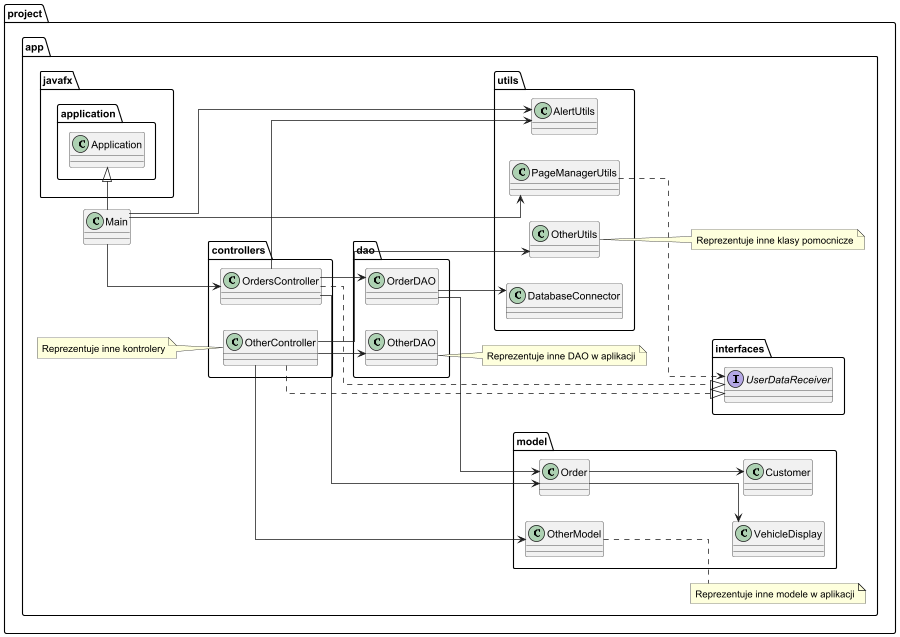
\includegraphics[height=0.4\textheight]{figures/diagramUML.png}
    \caption{Diagram UML}
    \label{fig:diagramUML}
\end{figure}

\newpage
\section{Pakiet resources - widoki graficzne i zasoby pomocnicze}

Pakiet \texttt{resources} zawiera wszystkie pliki niezbędne do prezentacji graficznej interfejsu użytkownika, a także dodatkowe zasoby wspierające działanie aplikacji. Struktura tego katalogu została podzielona na trzy główne grupy: pliki FXML, style CSS oraz multimedia (opcjonalne).

\subsection{Pliki FXML - definicje widoków}

Pliki z rozszerzeniem \texttt{.fxml} definiują strukturę graficznych interfejsów użytkownika aplikacji w oparciu o technologię JavaFX. Każdy plik odpowiada za konkretny ekran lub widok w aplikacji. Zostały one przygotowane z użyciem narzędzia Scene Builder i połączone z odpowiednimi kontrolerami.

\begin{table}[H]
\centering
\begin{tabular}{|p{4.5cm}|p{9.5cm}|}
\hline
\textbf{Plik FXML} & \textbf{Opis} \\
\hline
\texttt{customersPage.fxml} & Widok do zarządzania klientami: formularz dodawania klienta, tabela klientów. \\
\texttt{carsPage.fxml} & Widok listy pojazdów oraz formularz dodawania nowych aut. \\
\texttt{ordersPage.fxml} & Widok zleceń - umożliwia dodawanie i przeglądanie zleceń warsztatowych. \\
\texttt{servicesPage.fxml} & Widok zarządzania usługami serwisowymi. \\
\texttt{employeesPage.fxml} & Widok wyświetlania pracowników serwisu. \\
\texttt{loginPage.fxml} & Ekran logowania do aplikacji. \\
\hline
\end{tabular}
\caption{Pliki FXML i ich przeznaczenie}
\end{table}

\subsection{Pozostałe zasoby}

W folderze \texttt{resources} mogą znajdować się także dodatkowe podkatalogi z multimediami:

\begin{itemize}
    \item \texttt{values/} - pliki CSS definiujące styl graficzny aplikacji. Wpływają one na kolorystykę, wygląd przycisków, tabel oraz efektów interaktywnych.
    \item \texttt{images/} - ikony wykorzystywane w aplikacji.
\end{itemize}
Wszystkie ikony użyte w aplikacji pochodzą z serwisu Icons8. Tło oraz logo zostały opracowane na zamówienie.

\newpage
\section{Zarządzanie danymi i bazą danych}
\label{sec:zarzadzanieDanymi}

\subsection{Struktura encji i relacje}
W projekcie zastosowano relacyjną bazę danych, która przechowuje informacje niezbędne do zarządzania serwisem samochodowym. Główne encje (tabele) odzwierciedlają kluczowe obiekty systemu, takie jak: Klienci, Pojazdy, Pracownicy, Zlecenia, Usługi oraz Części.

Relacje między encjami są zaprojektowane zgodnie z zasadami normalizacji, aby uniknąć redundancji danych i zapewnić integralność. Przykładowo:

\begin{itemize}
    \item Jeden klient może posiadać wiele pojazdów (relacja 1 do N).
    \item Każde zlecenie jest powiązane z dokładnie jednym pojazdem i jednym pracownikiem odpowiedzialnym za realizację.
    \item Usługi oraz części są przypisane do zleceń, co pozwala na precyzyjne rozliczenie kosztów naprawy.
\end{itemize}


\begin{figure}[H]
    \centering
    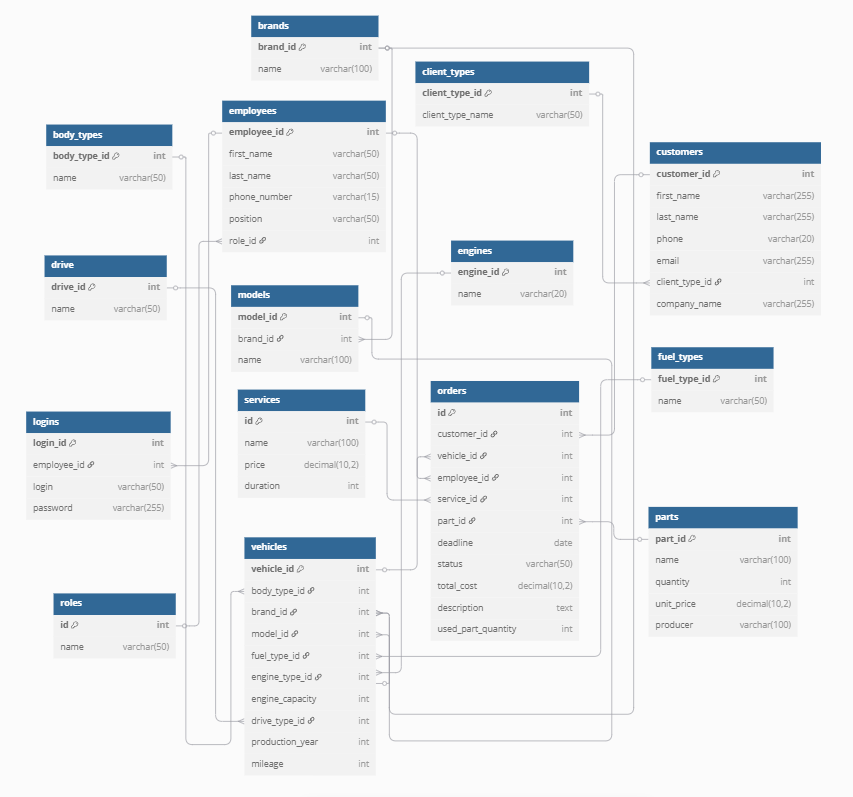
\includegraphics[width=0.7\textwidth,height=0.7\textheight,keepaspectratio]{figures/diagramERD.png}
    \caption{Diagram ERD bazy danych \texttt{warsztat}}
    \label{fig:diagramERD}
\end{figure}


\subsection{Opis przykładowych tabel}

\begin{itemize}
    \item Klienci - Tabela zawiera dane klientów: imię, nazwisko, numer telefonu, adres e-mail, typ klienta (osoba prywatna lub firma) oraz, w przypadku firm, nazwę przedsiębiorstwa.
    \item Samochody - Przechowuje informacje o samochodach powiązanych z klientami, takie jak marka, model, typ nadwozia, rodzaj paliwa, pojemność silnika, napęd oraz przebieg.
    \item Pracownicy - Dane o pracownikach serwisu, w tym imię, nazwisko oraz stanowisko.
    \item Zlecenia - Rejestruje pojedyncze naprawy, zawierając powiązania do klienta, pojazdu, pracownika, usługi i części. Zawiera także informacje o statusie i terminie realizacji.
\end{itemize}

\subsection{Relacje między tabelami}

Struktura bazy danych opiera się na kluczach głównych (PK) i obcych (FK), które definiują powiązania między tabelami. Najważniejsze relacje to:

\begin{itemize}
  \item \texttt{Pojazdy} (PK: \texttt{car\_id}) $\rightarrow$ \texttt{Zlecenia} (FK: \texttt{car\_id}),
  \item \texttt{Pracownicy} (PK: \texttt{employee\_id}) $\rightarrow$ \texttt{Zlecenia} (FK: \texttt{employee\_id}),
  \item \texttt{Usługi} oraz \texttt{Części} powiązane są z \texttt{Zleceniami} przez odpowiednie klucze,
\end{itemize}

Relacje zostały zaprojektowane tak, by zapewnić spójność i umożliwić łatwe rozszerzanie systemu.

\subsection{Podsumowanie}

Baza danych została zaprojektowana z myślą o przejrzystości i wydajności. Struktura encji i relacji gwarantuje integralność danych, minimalizuje ryzyko błędów oraz umożliwia sprawne zarządzanie informacjami w serwisie samochodowym. Takie podejście pozwala na łatwą rozbudowę funkcjonalności i utrzymanie systemu w przyszłości.